\documentclass[a4paper,11pt]{article}

%Headers
\usepackage[dvips]{graphicx}    %package that does pdfs
\usepackage{color}              %this needs to be here also
\usepackage{ulem}
\usepackage{amsmath}
\usepackage{pgfplots}
\usepackage{adjustbox}
\usepackage{graphicx}
\usepackage{enumitem}
\usepackage{listings}
\usepackage{tikz}
\usepackage{fancyvrb}
\usepackage{upquote}

\newcommand*\circled[1]{\tikz[baseline=(char.base)]{
             \node[shape=circle,draw,inner sep=2pt] (char) {#1};}}
\newcommand{\mybf}[1]{\boldsymbol{#1}}
\newcommand{\norm}[1]{\lvert\lvert #1 \rvert\rvert}

\title{%
	Problem Set 6\\
	\large MIT CW Linear Algebra (18.06)
}
\author{Aviel Livay}
\date{\today}

\begin{document}
\maketitle

\subsection*{Section 4.3, question 4}
\begin{align*}
&E=\norm{A\mybf{x}-b}^2=(C-1)^2+(C+D-8)^2+(C+3D-8)^2+(C+4D-20)^2 \\
\frac{\partial E}{\partial C} &= 2(C-1)+2(C+D-8)+2(C+3D-8)+2(C+4D-20) = 8C+16D-72=0 \\
\frac{\partial E}{\partial D} &= 2(C+D-8)+2(C+3D-8)*3+2(C+4D-20)*4 = 16C+52D-224=0 \\
\end{align*}
or in other words (and after dividing by 2)
\begin{align*}
4C+8D&=36 \\
8C+26D&=112 \\
\end{align*}
Using linear algebra:
\begin{align*}
A = 
\begin{bmatrix}
1 & 0 \\
1 & 1 \\
1 & 3 \\
1 & 4 \\
\end{bmatrix} \\
\end{align*}
\begin{align*}
A^TA\mybf{x}&=A^T\mybf{b} \\
\begin{bmatrix}
4 & 8 \\
8 & 26 \\
\end{bmatrix}
*
\begin{bmatrix}
C \\
D \\
\end{bmatrix}
&=
\begin{bmatrix}
1 & 1 & 1 & 1 \\
0 & 1 & 3 & 4 \\
\end{bmatrix} 
*
\begin{bmatrix}
0 \\
8 \\
8 \\
20 \\
\end{bmatrix} \\
\begin{bmatrix}
4 & 8 \\
8 & 26 \\
\end{bmatrix}
*
\begin{bmatrix}
C \\
D \\
\end{bmatrix}
&=
\begin{bmatrix}
36 \\
112 \\
\end{bmatrix} 
\end{align*}
\subsection*{Section 4.3, question 7}
\begin{align*}
A = 
\begin{bmatrix}
0 \\
1 \\
3 \\
4 \\
\end{bmatrix} \\
\end{align*}
\begin{align*}
A^TA\mybf{x}&=A^T\mybf{b} \\
26 * D &= 
\begin{bmatrix}
0 & 1 & 3 & 4 \\
\end{bmatrix} 
*
\begin{bmatrix}
0 \\
8 \\
8 \\
20 \\
\end{bmatrix} \\
26 * D &= 112
D = \frac{56}{13}
\end{align*}

\begin{adjustbox}{center}
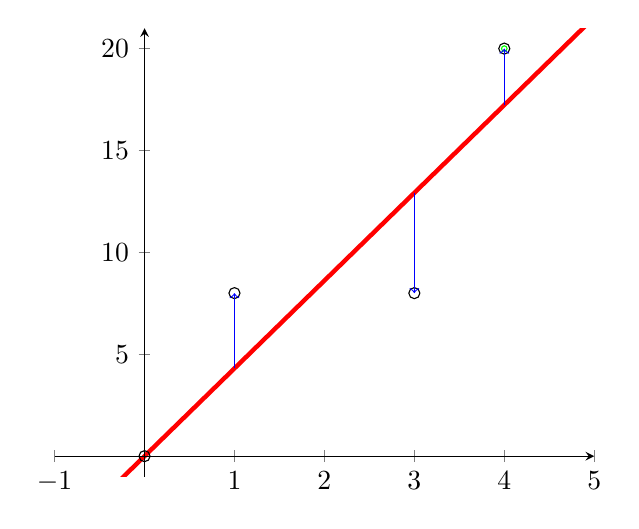
\begin{tikzpicture}
\begin{axis}[
    xmin=-1, xmax=5,
    ymin=-1, ymax=21,
    axis lines=center,
    axis on top=true,
    domain=-5:10,
    ]
    \addplot [mark=none,draw=red,ultra thick] {56/13*x};
    after end axis/.code={
    		   \draw (axis cs:0,0) circle (2pt);
               \draw (axis cs:1,8) circle (2pt);
               \draw (axis cs:3,8) circle (2pt);
               \draw (axis cs:4,20) circle (2pt);
               \draw [green](4,20) circle (1pt);   
               \draw[blue,->] (axis cs:1,56/13*1) -- (axis cs:1,8); 
               \draw[blue,->] (axis cs:3,56/13*3) -- (axis cs:3,8);
               \draw[blue,->] (axis cs:4,56/13*4) -- (axis cs:4,20);        
               }]
\end{axis}
\end{tikzpicture}
\end{adjustbox}

\subsection*{Section 4.3, question 9}
\begin{align*}
A = 
\begin{bmatrix}
1 & 0 & 0\\
1 & 1 & 1\\
1 & 3 & 9\\
1 & 4 & 16\\
\end{bmatrix} \\
\end{align*}
\begin{align*}
A^TA\mybf{x}&=A^T\mybf{b} \\
\begin{bmatrix}
4 & 8 & 26 \\
8 & 26 & 92\\
26 & 92 & 338\\
\end{bmatrix}
*
\begin{bmatrix}
C \\
D \\
E \\
\end{bmatrix}
&=
\begin{bmatrix}
1 & 1 & 1 & 1 \\
0 & 1 & 3 & 4 \\
0 & 1 & 9 & 16 \\
\end{bmatrix} 
*
\begin{bmatrix}
0 \\
8 \\
8 \\
20 \\
\end{bmatrix} \\
\begin{bmatrix}
4 & 8 & 26 \\
8 & 26 & 92\\
26 & 92 & 338\\
\end{bmatrix}
*
\begin{bmatrix}
C \\
D \\
E \\
\end{bmatrix}
&=
\begin{bmatrix}
36 \\
112 \\
400 \\
\end{bmatrix} \\
\end{align*}
Solving in Octave gives: $\mybf{x}=(2, \frac{4}{3}, \frac{2}{3})$

\begin{adjustbox}{center}
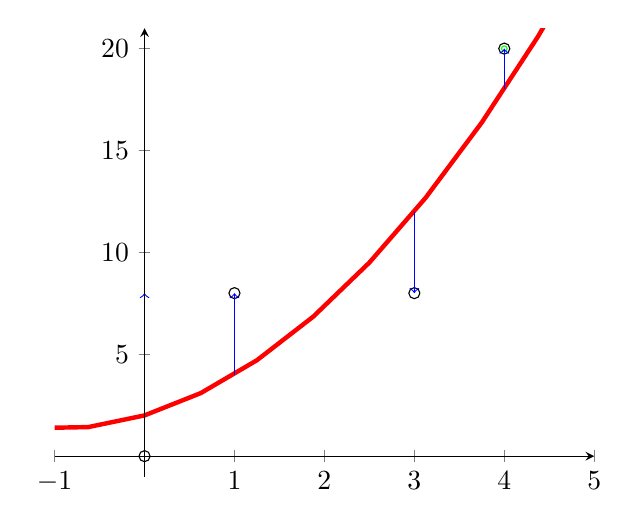
\begin{tikzpicture}
\begin{axis}[
    xmin=-1, xmax=5,
    ymin=-1, ymax=21,
    axis lines=center,
    axis on top=true,
    domain=-5:10,
    ]
    \addplot [mark=none,draw=red,ultra thick] {2+4/3*x+2/3*x^2};
    after end axis/.code={
    		   \draw (axis cs:0,0) circle (2pt);
               \draw (axis cs:1,8) circle (2pt);
               \draw (axis cs:3,8) circle (2pt);
               \draw (axis cs:4,20) circle (2pt);
               \draw [green](4,20) circle (1pt);   
               \draw[blue,->] (axis cs:0,2+4/3*0+2/3*0^2) -- (axis cs:0,8);
               \draw[blue,->] (axis cs:1,2+4/3*1+2/3*1^2) -- (axis cs:1,8); 
               \draw[blue,->] (axis cs:3,2+4/3*3+2/3*3^2) -- (axis cs:3,8);
               \draw[blue,->] (axis cs:4,2+4/3*4+2/3*4^2) -- (axis cs:4,20);        
               }]
\end{axis}
\end{tikzpicture}
\end{adjustbox}
Nothing much is changed in figure 4.9b except for the fact that now p is now a linear combination of 3 vectors with $p$ having more options to get closer to $b$.
\subsection*{Section 4.3, question 26}
\begin{align*}
C+D+0 = 0 \\
C+0+E = 1 \\
C-D+0 = 3 \\
C+0-E = 4 \\
\end{align*}
\begin{align*}
A = 
\begin{bmatrix}
1 & 1 & 0 \\
1 & 0 & 1 \\
1 & -1 & 0 \\
1 & 0 & -1 \\
\end{bmatrix}
\end{align*}
And we are trying to solve:
\begin{align*} 
\begin{bmatrix}
1 & 1 & 0 \\
1 & 0 & 1 \\
1 & -1 & 0 \\
1 & 0 & -1 \\
\end{bmatrix}
\mybf{x} =
\begin{bmatrix}
0 \\
1\\
3 \\
4 \\
\end{bmatrix}
\end{align*}
But since there's no solution then we are trying to solve instead $A^TA\mybf{x}=A^T\mybf{b}$ and we get $\mybf{x}=(2,-1.5, -1.5)$ so the equation of the plane is $2-3x-3y=0$. It gives $(-1, -1, 5, 5)$ as best approximation for $(0,1,3,4)$ values on the corners. At the center, which is not on the plane, we get $2-3x-3y=2-3*0-3*0=2$ which is the average of $(0,1,3,4)$
\begin{adjustbox}{center}
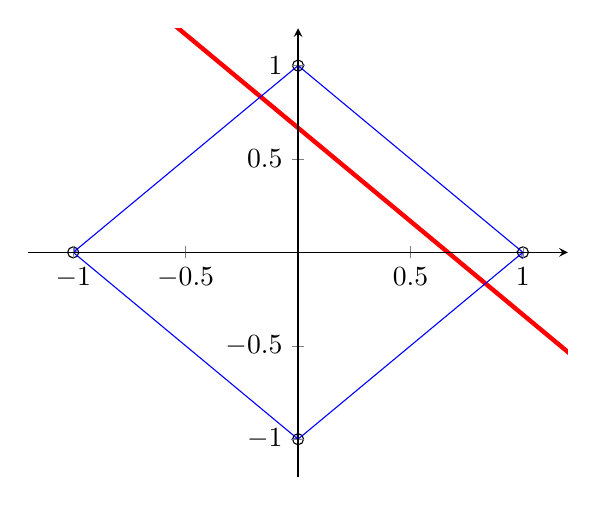
\begin{tikzpicture}
\begin{axis}[
    xmin=-1.2, xmax=1.2,
    ymin=-1.2, ymax=1.2,
    axis lines=center,
    axis on top=true,
    domain=-1.5:1.5,
    ]
    \addplot [mark=none,draw=red,ultra thick] {(2-3*x)/3};
    after end axis/.code={
    		   \draw (axis cs:1,0) circle (2pt);
               \draw (axis cs:0,1) circle (2pt);
               \draw (axis cs:-1,0) circle (2pt);
               \draw (axis cs:0,-1) circle (2pt);
               \draw[blue,->] (axis cs:1,0) -- (axis cs:0,1);
               \draw[blue,->] (axis cs:0,1) -- (axis cs:-1,0); 
               \draw[blue,->] (axis cs:-1,0) -- (axis cs:0,-1);
               \draw[blue,->] (axis cs:0,-1) -- (axis cs:1,0);        
               }]
\end{axis}
\end{tikzpicture}
\end{adjustbox}
\subsection*{Section 4.3, question 29}
Example for $n=3$: there will be one plane containing $0$, $a_1$, $a_2$ unless $a_1$ and $a_2$ are linearly dependent in which case they represent one vector  which can be part of many planes, not just one.\\
As for $R^N$, if we take the $n-1$ points and connect each one to the 0 point then we end up with $n-1$ vectors. if $A$ is the matrix which columns are the vectors, then if that matrix has a rank of $n-1$ then there's only one single vector that's in the null space and is perpendicular to all of the columns. The unique plane is orthogonal to this vector. So this is true only if indeed all vectors to all the $n-1$ points are linearly independent. 
\subsection*{Section 4.4, question 10}
\begin{enumerate}
\item The definition of orthonormal vectors is that $\mybf{q_i}\cdot\mybf{q_j}=0$ for $i ne j$ and equal $1$ for $i=j$.
for $c_1=0$, $c_2=0$ and $c_3=0$ we have the following equations:
\begin{align*}
&&c_2\mybf{q_2}+&&c_3\mybf{q_3}&&=0\\
&c_1\mybf{q_1}+&&&c_3\mybf{q_3}&&=0\\
&c_1\mybf{q_1}+&c_2\mybf{q_2}&&&&=0\\
\end{align*}
The only solution for this set of equations is $c_1=c_2=c_3=0$.
\item 
\begin{align*}
Q\mybf{x}&=\mybf{0} \\
Q^TQ\mybf{x}&=Q^T\mybf{0} \\
I\mybf{x}&=\mybf{0} \\
\mybf{x}&=0
\end{align*}
Since the only solution to the equation $Q\mybf{x}=\mybf{0}$ is $\mybf{x}=\mybf{0}$ which means that the vectors of $Q$ are linearly independent and therefore $q_i$'s are linearly independent.
\end{enumerate}
\subsection*{Section 4.4, question 18}
Starting with $\mybf{a}=(1,-1,0,0)$, $\mybf{b}=(0,1,-1,0)$, $\mybf{c}=(0,0,1,-1)$.
We start with $a$ and we don't touch it. It's good enough as is.
We now subtract $B$'s projection along $A$ leaving us with the perpendicular part which is orthogonal to $a$.
\begin{align*}
B=b-\frac{A^Tb}{A^TA}A.
\end{align*}
\begin{align*}
A^Tb=
\begin{bmatrix}
1 & -1 & 0 & 0 \\
\end{bmatrix}
*
\begin{bmatrix}
0 \\
1 \\
-1 \\
0 \\
\end{bmatrix}
= -1
\end{align*}
\begin{align*}
A^TA=
\begin{bmatrix}
1 & -1 & 0 & 0 \\
\end{bmatrix}
*
\begin{bmatrix}
1 \\
-1 \\
0 \\
0 \\
\end{bmatrix}
= 2
\end{align*}
\begin{align*}
B=b-\frac{A^Tb}{A^TA}A= 
\begin{bmatrix}
0 \\
1 \\
-1 \\
0 \\
\end{bmatrix}
-
\frac{-1}{2}*
\begin{bmatrix}
1 \\
-1 \\
0 \\
0 \\
\end{bmatrix}
=
\begin{bmatrix}
\frac{1}{2} \\
\frac{1}{2} \\
-1 \\
0 \\
\end{bmatrix}
\end{align*}
and now we move to the third vector:
$C=c-\frac{A^Tc}{A^TA}A-\frac{B^Tc}{B^TB}B$.
\begin{align*}
A^Tc=
\begin{bmatrix}
1 & -1 & 0 & 0 \\
\end{bmatrix}
*
\begin{bmatrix}
0 \\
0 \\
1 \\
-1 \\
\end{bmatrix}
= 0
\end{align*}
\begin{align*}
B^Tc=
\begin{bmatrix}
\frac{1}{2} & \frac{1}{2} & -1 & 0 \\
\end{bmatrix}
*
\begin{bmatrix}
0 \\
0 \\
1 \\
-1 \\
\end{bmatrix}
= -1
\end{align*}
\begin{align*}
C=c-\frac{A^Tc}{A^TA}A-\frac{B^Tc}{B^TB}B=c-\frac{B^Tc}{B^TB}B=
\begin{bmatrix}
0 \\
0 \\
1 \\
-1 \\
\end{bmatrix}
-
\frac{-1}{1.5}*
\begin{bmatrix}
\frac{1}{2} \\
\frac{1}{2} \\
-1 \\
0 \\
\end{bmatrix}
=
\begin{bmatrix}
\frac{1}{3} \\
\frac{1}{3} \\
\frac{1}{3} \\
-1 \\
\end{bmatrix}
\end{align*}
So $A=(1,-1,0,0)$, $B=(\frac{1}{2}, \frac{1}{2}, -1, 0)$ and $C=(\frac{1}{3},\frac{1}{3},\frac{1}{3},1)$. 
We can now normalize these vectors and get:
$A=(\frac{1}{\sqrt{2}},-\frac{1}{\sqrt{2}},0,0)$, $B=(\frac{1}{\sqrt{6}}, \frac{1}{\sqrt{6}}, -\sqrt{\frac{2}{3}}, 0)$ and $C=(\frac{1}{2\sqrt{3}},\frac{1}{2\sqrt{3}},\frac{1}{2\sqrt{3}},-\frac{3}{\sqrt{2}})$.
\subsection*{Section 4.4, question 35}
After calculating the QR decomposition in MATLAB - I get 
\begin{align*}
\begin{bmatrix}
-\frac{1}{\sqrt{2}} & -\frac{1}{\sqrt{6}} & -\frac{1}{\sqrt{12}} & \frac{1}{2}\\
\frac{1}{\sqrt{2}} & -\frac{1}{\sqrt{6}} & -\frac{1}{\sqrt{12}} & \frac{1}{2}\\
0 & \frac{2}{\sqrt{6}} & -\frac{1}{\sqrt{12}} & \frac{1}{2}\\
0 & 0 & \frac{3}{\sqrt{12}} & \frac{1}{2}\\
\end{bmatrix}
\end{align*}
The question is not very clear. \\
If you want to get rid of the $\sqrt{2}$ which is the denominator of the first column then you just multiply by $\sqrt{2}$. Trivial.
If you want to scale all the columns by the same constant, then if we take a look at the denominators after multiplying all by $-2$, then we see: $\frac{1}{\sqrt{2}}$, $\frac{1}{\sqrt{2}\sqrt{3}}$, $\frac{1}{\sqrt{3}}$ and $1$
For the first column we need to multiply by an integer multiplied by ${\sqrt{2}^i}$ where $i$ is odd. For the second column we need in addition to multiply by an integer multiplied by ${\sqrt{3}^j}$ where $j$ is odd so this is impossible.\\
If you want to multiply each column separately but you want the columns to remain orthonormal, this is impossible since QR decomposition is unique except for a multiplying by a diagonal matrix with $-1$, $+1$ on the diagonal.
\subsection*{Section 4.4, question 36}
\begin{enumerate}
\item The $n$ columns of $Q_1$ are the orthonormal basis for the columns of $A$.
\item The $m-n$ columns of $Q_2$ are continuing the Gram-Schmidt process and generating vectors that are orthogonal to the vectors in the columns of A. Which means they are creating an orthonormal basis for the left null space of A.
\end{enumerate}
\subsection*{Section 5.1, question 10}
The solution is simple: $\mybf{x}=(1,1,1)$ so indeed $\text{det}A=0$. If all the entries are summed to 1 then it means that $A*(1,1,1)=(1,1,1)$ which means that $(A-I)*(1,1,1)=(0,0,0)$ which proves that $A-I$ is singular so $\text{det}(A-I)=0$. It doesn't mean that $\text{det}A=1$ because $A$ could be equal for example to 
\begin{align*}
\begin{bmatrix}
2 & -1 \\
3 & -2 \\
\end{bmatrix}
\end{align*}
then indeed the sum of all lines is one but $\text{det}A=0\ne1$
\subsection*{Section 5.1, question 18}
\begin{align*}
\text{det}
\begin{bmatrix}
1 & a & a^2 \\
1 & b & b^2 \\
1 & c & c^2 \\
\end{bmatrix}
\end{align*}
\begin{align*}
\text{det}
\begin{bmatrix}
1 & a & a^2 \\
0 & b-a & b^2-a^2 \\
0 & c-a & c^2-a^2 \\
\end{bmatrix}
\end{align*}
\begin{align*}
\text{det}
\begin{bmatrix}
1 & a & a^2 \\
0 & b-a & b^2-a^2 \\
0 & 0 & (c-a)(c-b) \\
\end{bmatrix}
\end{align*}
This upper triangular matrix has $1$, $b-a$ and $(c-a)(c-b)$ on the diagonal so the determinant is the multiplication of those: $(b-a)(c-a)(c-b)$.
\subsection*{Section 5.1, question 31}
>> det(hilb(1))\\
ans = 1\\
>> det(hilb(2))\\
ans = 0.083333\\
>> det(hilb(3))\\
ans = 4.6296e-04\\
>> det(hilb(4))\\
ans = 1.6534e-07\\
>> det(hilb(5))\\
ans = 3.7493e-12\\
>> det(hilb(6))\\
ans = 5.3673e-18\\
>> det(hilb(7))\\
ans = 4.8358e-25\\
>> det(hilb(8))\\
ans = 2.7371e-33\\
>> det(hilb(9))\\
ans = 9.7203e-43\\
>> det(hilb(10))\\
ans = 2.1644e-53\\
>> rref(hilb(5))\\
ans =\\
\\
   1   0   0   0   0\\
   0   1   0   0   0\\
   0   0   1   0   0\\
   0   0   0   1   0\\
   0   0   0   0   1\\
\subsection*{Section 5.1, question 32}
if we denote by $F(n)$ the maximum determinant of a matrix rand(n) then we can say that such a matrix has a determinant between 0 and $F(n)$.
So trivially $F(1)=1$.
And the 'induction stage' is that $F(n)=n*F(n-1)$ because the determinant can be calculated by going over all the elements of the first row and multiply by the determinants of the matrices (n-1)x(n-1).
So basically F(4) for example gets values between 0 and 4!=24.
$\text{det}A_{1x1}$ is a number between 0 and 1.
$\text{det}A_{2x2}=a$ is a number between 0 and 1.
Determinant of 2x2 matrix is an addition of 2 determinants of 1x1 matrices multiplied each by a number between
\end{document}